%%
%% Beginning of file 'sample62.tex'
%%
%% Modified 2018 January
%%
%% This is a sample manuscript marked up using the
%% AASTeX v6.2 LaTeX 2e macros.
%%
%% AASTeX is now based on Alexey Vikhlinin's emulateapj.cls 
%% (Copyright 2000-2015).  See the classfile for details.

%% AASTeX requires revtex4-1.cls (http://publish.aps.org/revtex4/) and
%% other external packages (latexsym, graphicx, amssymb, longtable, and epsf).
%% All of these external packages should already be present in the modern TeX 
%% distributions.  If not they can also be obtained at www.ctan.org.

%% The first piece of markup in an AASTeX v6.x document is the \documentclass
%% command. LaTeX will ignore any data that comes before this command. The 
%% documentclass can take an optional argument to modify the output style.
%% The command below calls the preprint style  which will produce a tightly 
%% typeset, one-column, single-spaced document.  It is the default and thus
%% does not need to be explicitly stated.
%%
%%
%% using aastex version 6.2
\documentclass[modern]{aastex62}

%% The default is a single spaced, 10 point font, single spaced article.
%% There are 5 other style options available via an optional argument. They
%% can be envoked like this:
%%
%% \documentclass[argument]{aastex62}
%% 
%% where the layout options are:
%%
%%  twocolumn   : two text columns, 10 point font, single spaced article.
%%                This is the most compact and represent the final published
%%                derived PDF copy of the accepted manuscript from the publisher
%%  manuscript  : one text column, 12 point font, double spaced article.
%%  preprint    : one text column, 12 point font, single spaced article.  
%%  preprint2   : two text columns, 12 point font, single spaced article.
%%  modern      : a stylish, single text column, 12 point font, article with
%% 		  wider left and right margins. This uses the Daniel
%% 		  Foreman-Mackey and David Hogg design.
%%  RNAAS       : Preferred style for Research Notes which are by design 
%%                lacking an abstract and brief. DO NOT use \begin{abstract}
%%                and \end{abstract} with this style.
%%
%% Note that you can submit to the AAS Journals in any of these 6 styles.
%%
%% There are other optional arguments one can envoke to allow other stylistic
%% actions. The available options are:
%%
%%  astrosymb    : Loads Astrosymb font and define \astrocommands. 
%%  tighten      : Makes baselineskip slightly smaller, only works with 
%%                 the twocolumn substyle.
%%  times        : uses times font instead of the default
%%  linenumbers  : turn on lineno package.
%%  trackchanges : required to see the revision mark up and print its output
%%  longauthor   : Do not use the more compressed footnote style (default) for 
%%                 the author/collaboration/affiliations. Instead print all
%%                 affiliation information after each name. Creates a much
%%                 long author list but may be desirable for short author papers
%%
%% these can be used in any combination, e.g.
%%
%% \documentclass[twocolumn,linenumbers,trackchanges]{aastex62}
%%
%% AASTeX v6.* now includes \hyperref support. While we have built in specific
%% defaults into the classfile you can manually override them with the
%% \hypersetup command. For example,
%%
%%\hypersetup{linkcolor=red,citecolor=green,filecolor=cyan,urlcolor=magenta}
%%
%% will change the color of the internal links to red, the links to the
%% bibliography to green, the file links to cyan, and the external links to
%% magenta. Additional information on \hyperref options can be found here:
%% https://www.tug.org/applications/hyperref/manual.html#x1-40003
%%
%% If you want to create your own macros, you can do so
%% using \newcommand. Your macros should appear before
%% the \begin{document} command.
%%
% added by DH
\newcommand{\numax}{\mbox{$\nu_{\rm max}$}\xspace}
\newcommand{\Dnu}{\mbox{$\Delta \nu$}\xspace}
\newcommand{\dnu}{\mbox{$\delta \nu$}\xspace}
\newcommand{\muHz}{\mbox{$\mu$Hz}\xspace}
\newcommand{\teff}{\mbox{$T_{\rm eff}$}\xspace}
\newcommand{\logg}{\mbox{$\log g$}\xspace}
\newcommand{\feh}{\mbox{$\rm{[Fe/H]}$}\xspace}
\newcommand{\msun}{\mbox{$\mathrm{M}_{\sun}$}\xspace}
\newcommand{\rsun}{\mbox{$\mathrm{R}_{\sun}$}\xspace}
\newcommand{\hipparcos}{\textit{Hipparcos}\xspace}
\newcommand{\gaia}{\textit{Gaia}\xspace}


\newcommand{\vdag}{(v)^\dagger}
\newcommand\aastex{AAS\TeX}
\newcommand\latex{La\TeX}
\newcommand\kepler{\emph{Kepler}\,}
\newcommand\ktwo{\emph{K2}\,}

\definecolor{linkcolor}{rgb}{0.1216,0.4667,0.7059}


\usepackage{xcolor, fontawesome}
\definecolor{twitterblue}{RGB}{64,153,255}
\newcommand\twitter[1]{\href{https://twitter.com/#1 }{\textcolor{twitterblue}{\faTwitter}\,\tt \textcolor{twitterblue}{@#1}}}


%% Tells LaTeX to search for image files in the 
%% current directory as well as in the figures/ folder.
\graphicspath{{../notebooks/}}

%% Reintroduced the \received and \accepted commands from AASTeX v5.2
\received{January 1, 2019}
\revised{January 7, 2019}
\accepted{\today}
%% Command to document which AAS Journal the manuscript was submitted to.
%% Adds "Submitted to " the arguement.
\submitjournal{ApJ}

%% Mark up commands to limit the number of authors on the front page.
%% Note that in AASTeX v6.2 a \collaboration call (see below) counts as
%% an author in this case.
%
%\AuthorCollaborationLimit=3
%
%% Will only show Schwarz, Muench and "the AAS Journals Data Scientist 
%% collaboration" on the front page of this example manuscript.
%%
%% Note that all of the author will be shown in the published article.
%% This feature is meant to be used prior to acceptance to make the
%% front end of a long author article more manageable. Please do not use
%% this functionality for manuscripts with less than 20 authors. Conversely,
%% please do use this when the number of authors exceeds 40.
%%
%% Use \allauthors at the manuscript end to show the full author list.
%% This command should only be used with \AuthorCollaborationLimit is used.

%% The following command can be used to set the latex table counters.  It
%% is needed in this document because it uses a mix of latex tabular and
%% AASTeX deluxetables.  In general it should not be needed.
%\setcounter{table}{1}

%%%%%%%%%%%%%%%%%%%%%%%%%%%%%%%%%%%%%%%%%%%%%%%%%%%%%%%%%%%%%%%%%%%%%%%%%%%%%%%%
%%
%% The following section outlines numerous optional output that
%% can be displayed in the front matter or as running meta-data.
%%
%% If you wish, you may supply running head information, although
%% this information may be modified by the editorial offices.
\shorttitle{No Giant Planet around GJ 1151}
\shortauthors{B. J. S. Pope et al.}
%%
%% You can add a light gray and diagonal water-mark to the first page 
%% with this command:
% \watermark{text}
%% where "text", e.g. DRAFT, is the text to appear.  If the text is 
%% long you can control the water-mark size with:
%  \setwatermarkfontsize{dimension}
%% where dimension is any recognized LaTeX dimension, e.g. pt, in, etc.
%%
%%%%%%%%%%%%%%%%%%%%%%%%%%%%%%%%%%%%%%%%%%%%%%%%%%%%%%%%%%%%%%%%%%%%%%%%%%%%%%%%

%% This is the end of the preamble.  Indicate the beginning of the
%% manuscript itself with \begin{document}.

\begin{document}

\title{No Giant Planet around Aurora Candidate GJ 1151}

\correspondingauthor{Benjamin J. S. Pope \twitter{fringetracker}}
\email{benjamin.pope@nyu}

\author[0000-0003-2595-9114]{Benjamin J. S. Pope}
\affiliation{Center for Cosmology and Particle Physics, Department of Physics, New York University, 726 Broadway, New York, NY 10003, USA}
\affiliation{NASA Sagan Fellow}

\author[0000-0002-8171-8596]{Megan Bedell}
\affiliation{Center for Computational Astrophysics, Flatiron Institute, 162 Fifth Ave, New York, NY 10010, USA}

\author[0000-0002-7167-1819]{Joseph R. Callingham}
\affiliation{ASTRON, Netherlands Institute for Radio Astronomy, Oude Hoogeveensedijk 4, Dwingeloo, 7991 PD, The Netherlands}

\author{friends}
%% Note that the \and command from previous versions of AASTeX is now
%% depreciated in this version as it is no longer necessary. AASTeX 
%% automatically takes care of all commas and "and"s between authors names.

%% AASTeX 6.2 has the new \collaboration and \nocollaboration commands to
%% provide the collaboration status of a group of authors. These commands 
%% can be used either before or after the list of corresponding authors. The
%% argument for \collaboration is the collaboration identifier. Authors are
%% encouraged to surround collaboration identifiers with ()s. The 
%% \nocollaboration command takes no argument and exists to indicate that
%% the nearby authors are not part of surrounding collaborations.

%% Mark off the abstract in the ``abstract'' environment. 
\begin{abstract}
We don't find a star or giant planet around GJ 1151 but we cannot rule out anything below 10 $M_\oplus$. 

We infer a high resolution spectrum of GJ 1151 which is pretty cool.
\href{https://github.com/benjaminpope/video}{\color{linkcolor}\faGithub} % shamelessly borrowed from Luger!

\end{abstract}

%% Keywords should appear after the \end{abstract} command. 
%% See the online documentation for the full list of available subject
%% keywords and the rules for their use.
% \keywords{editorials, notices --- 
% miscellaneous --- catalogs --- surveys}


\section{Introduction} 
\label{sec:intro}

Vedantham et al (submitted) have detected GJ~1151 at low radio frequencies with LOFAR, indicating a possible star-planet magnetic interaction analogous to Jupiter-Io.

\section{HARPS RV Data}
\label{sec:k2}

\begin{figure}
\noindent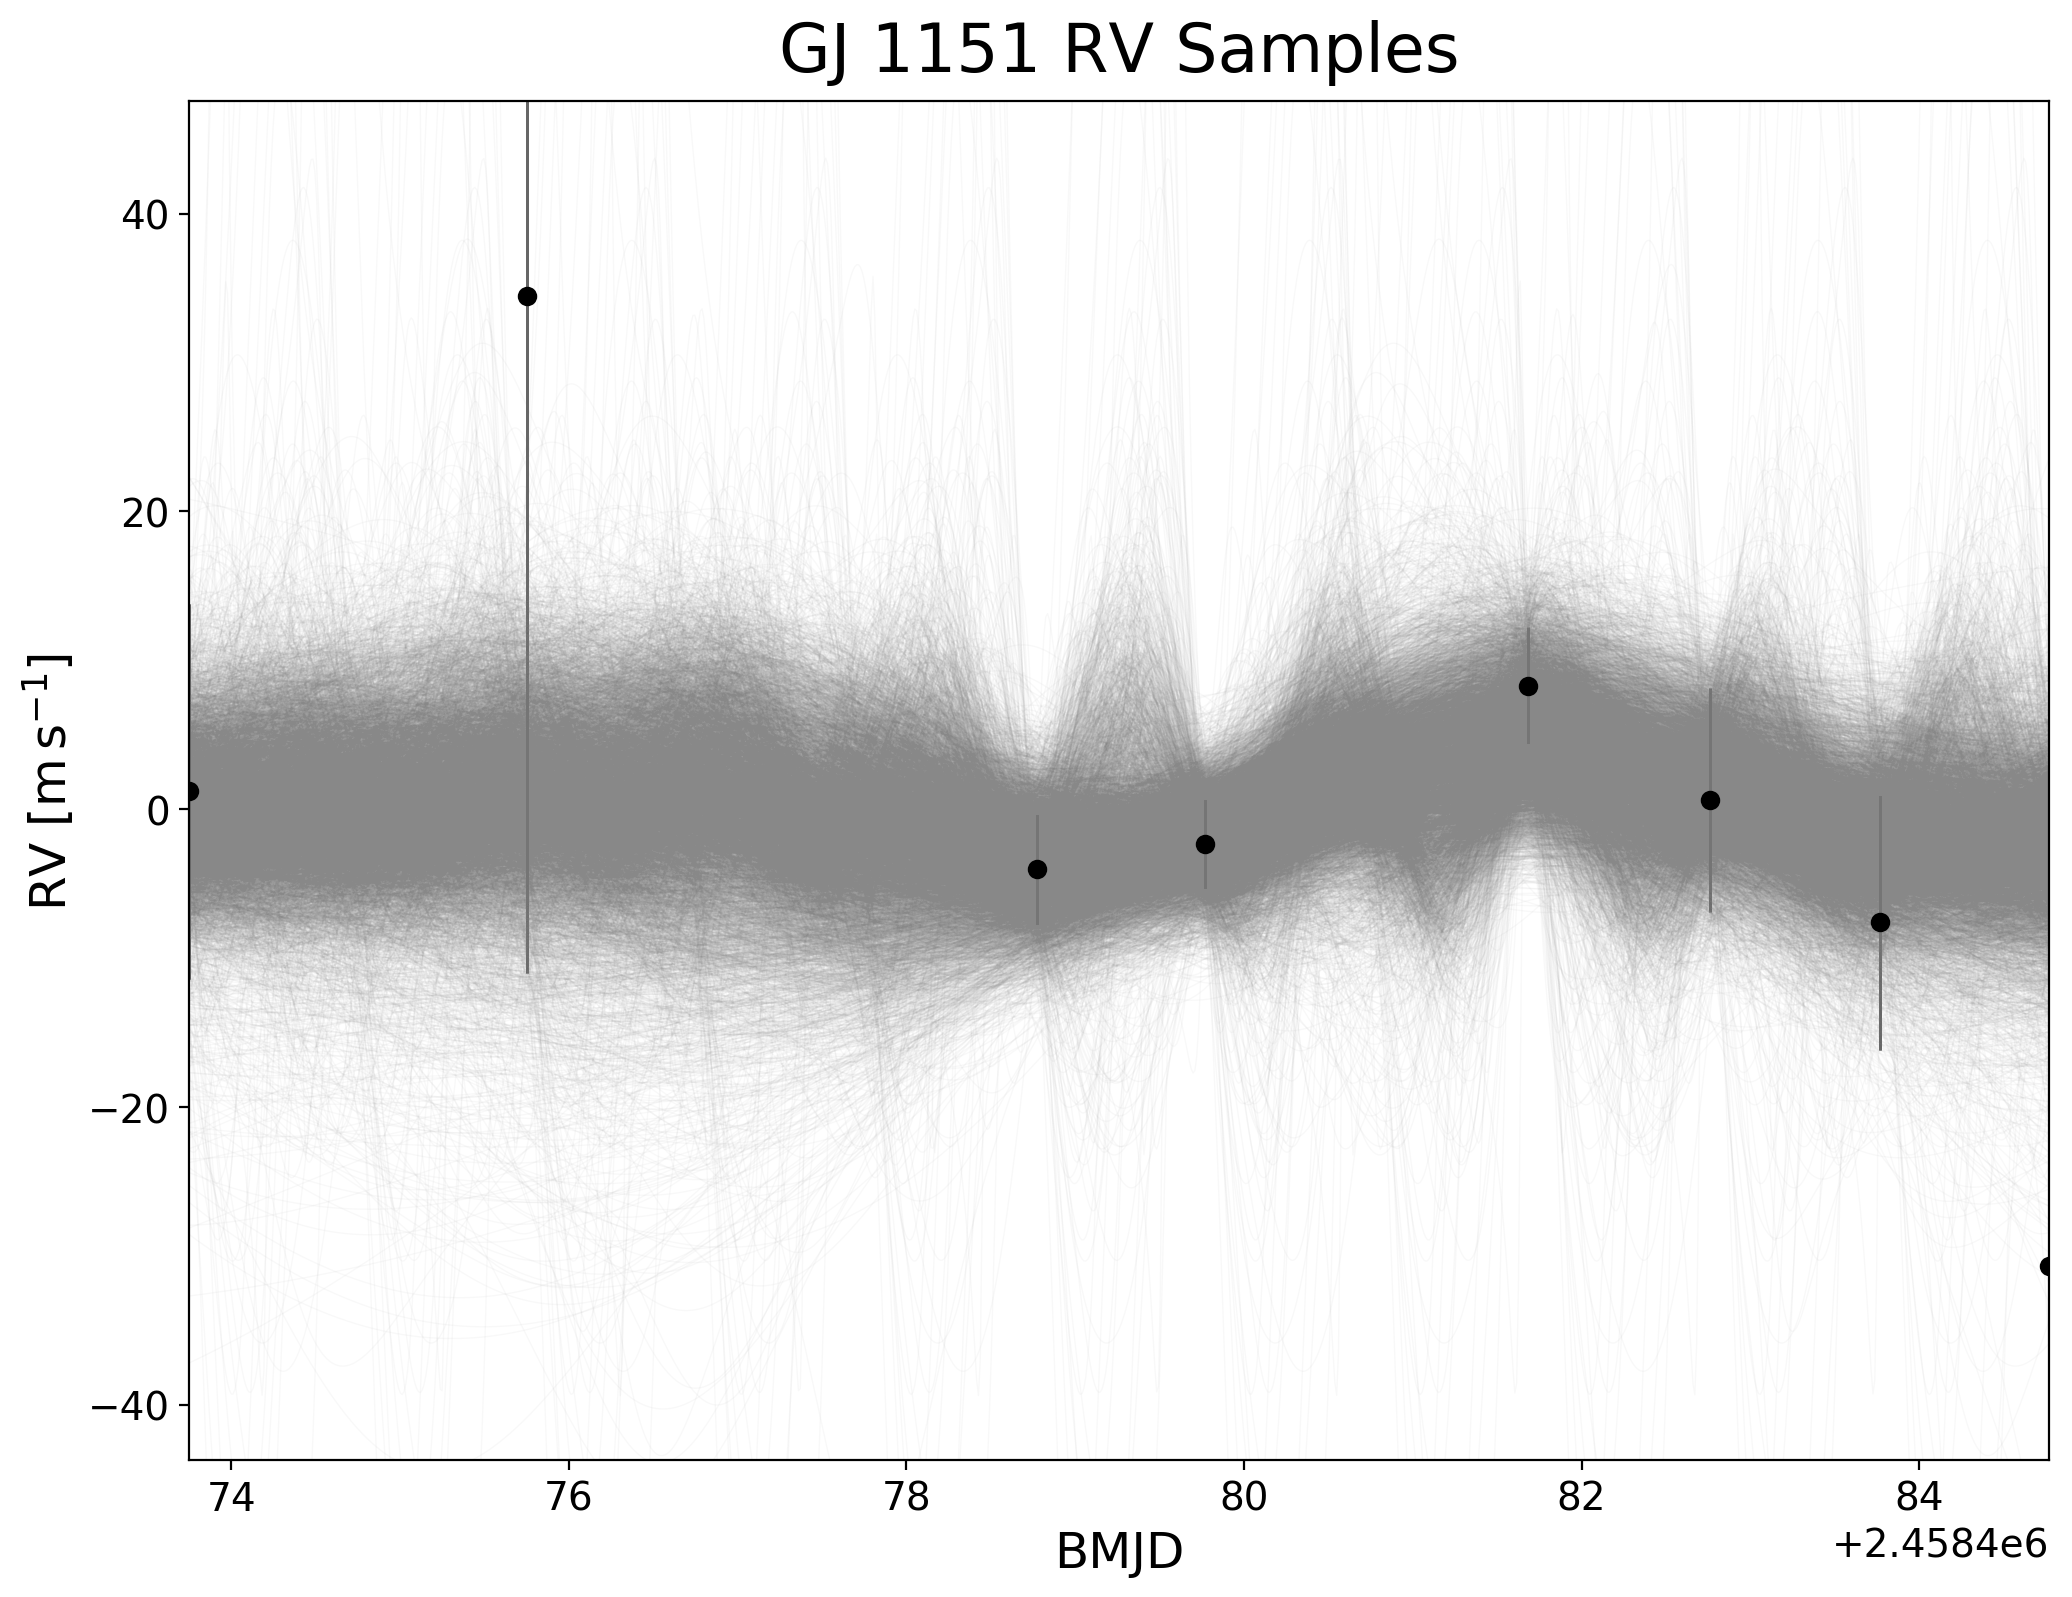
\includegraphics[width=15cm,keepaspectratio]{gj1151b_samples.png}

\caption{\label{jokermodel}
The Joker posterior samples.
}
\end{figure}

\begin{figure}
\noindent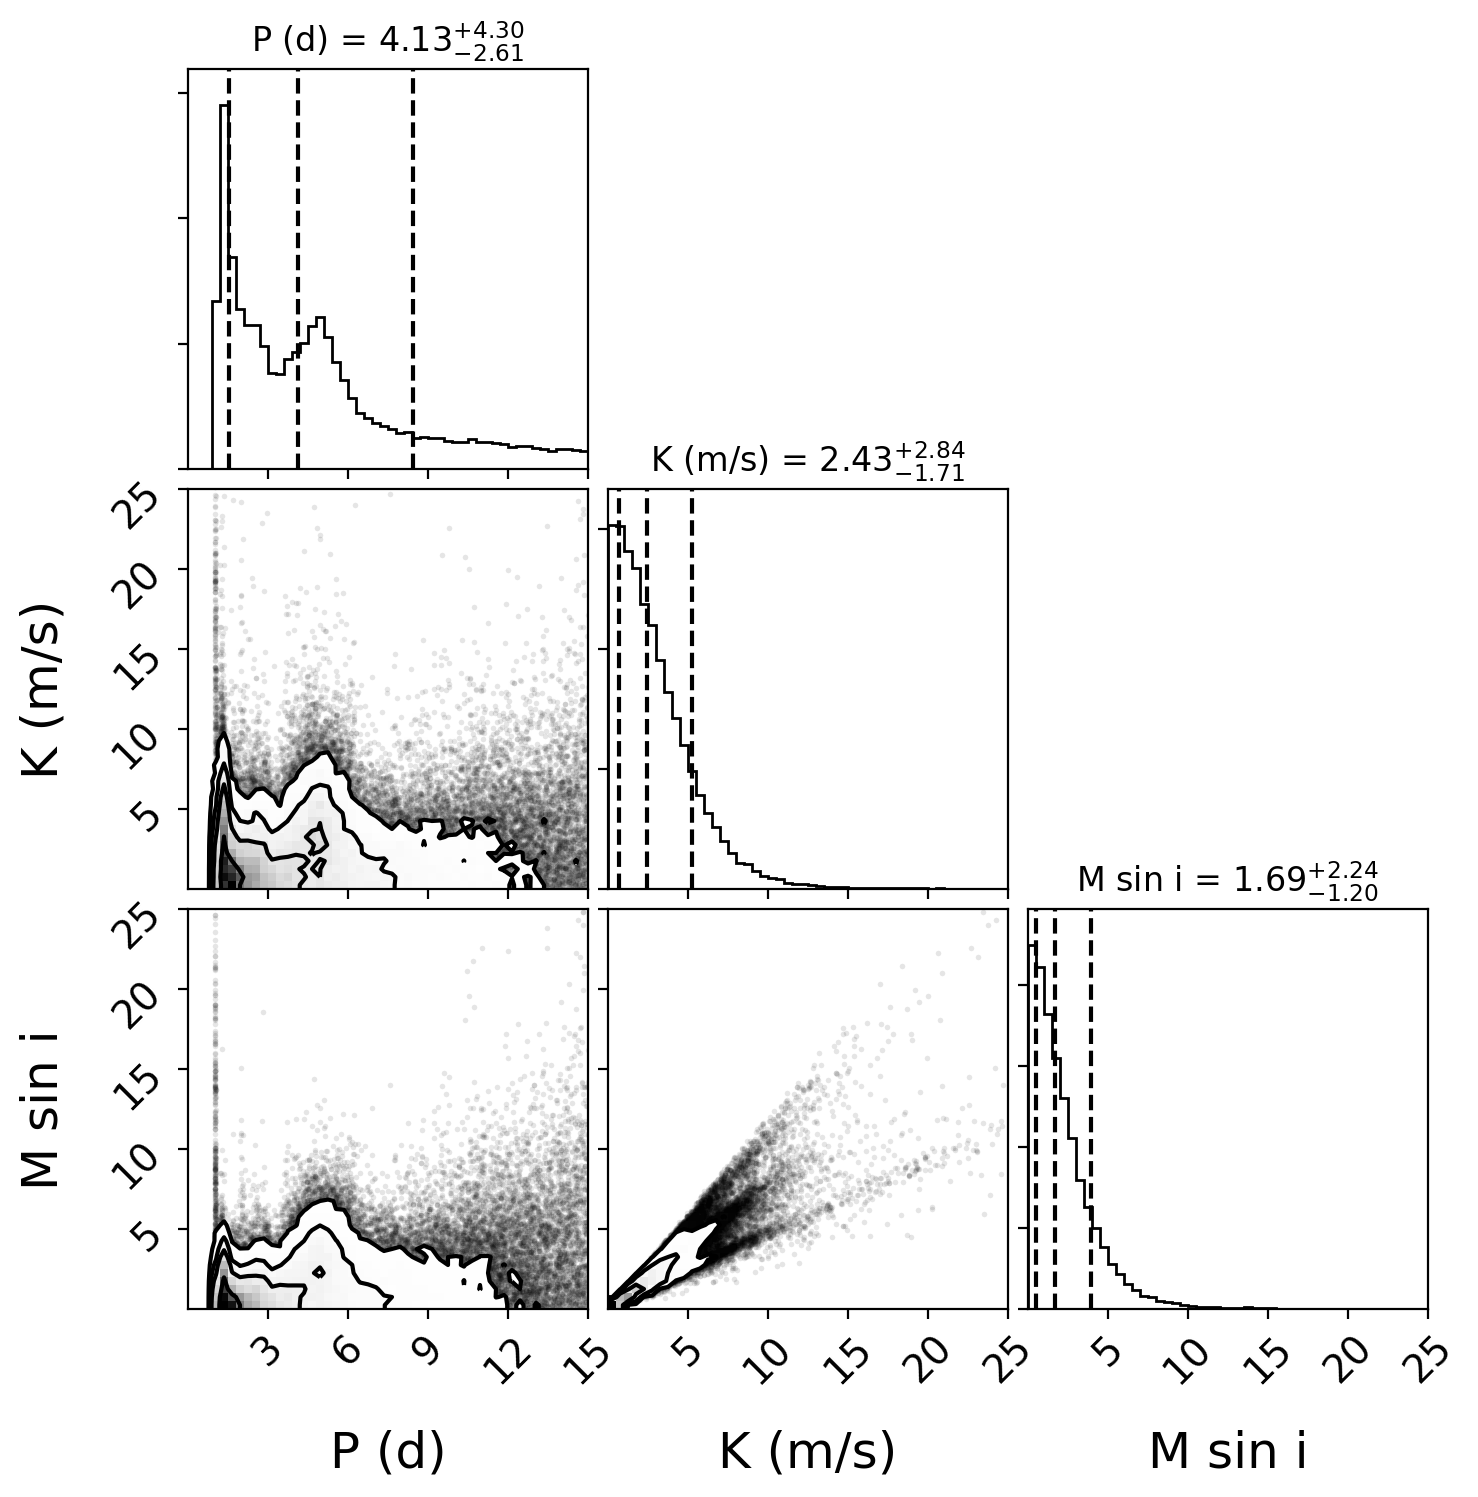
\includegraphics[width=15cm,keepaspectratio]{cornerplot_k.png}

\caption{\label{cornerplot}
Cornerplot of posterior from The Joker.
}
\end{figure}

\begin{figure}
\noindent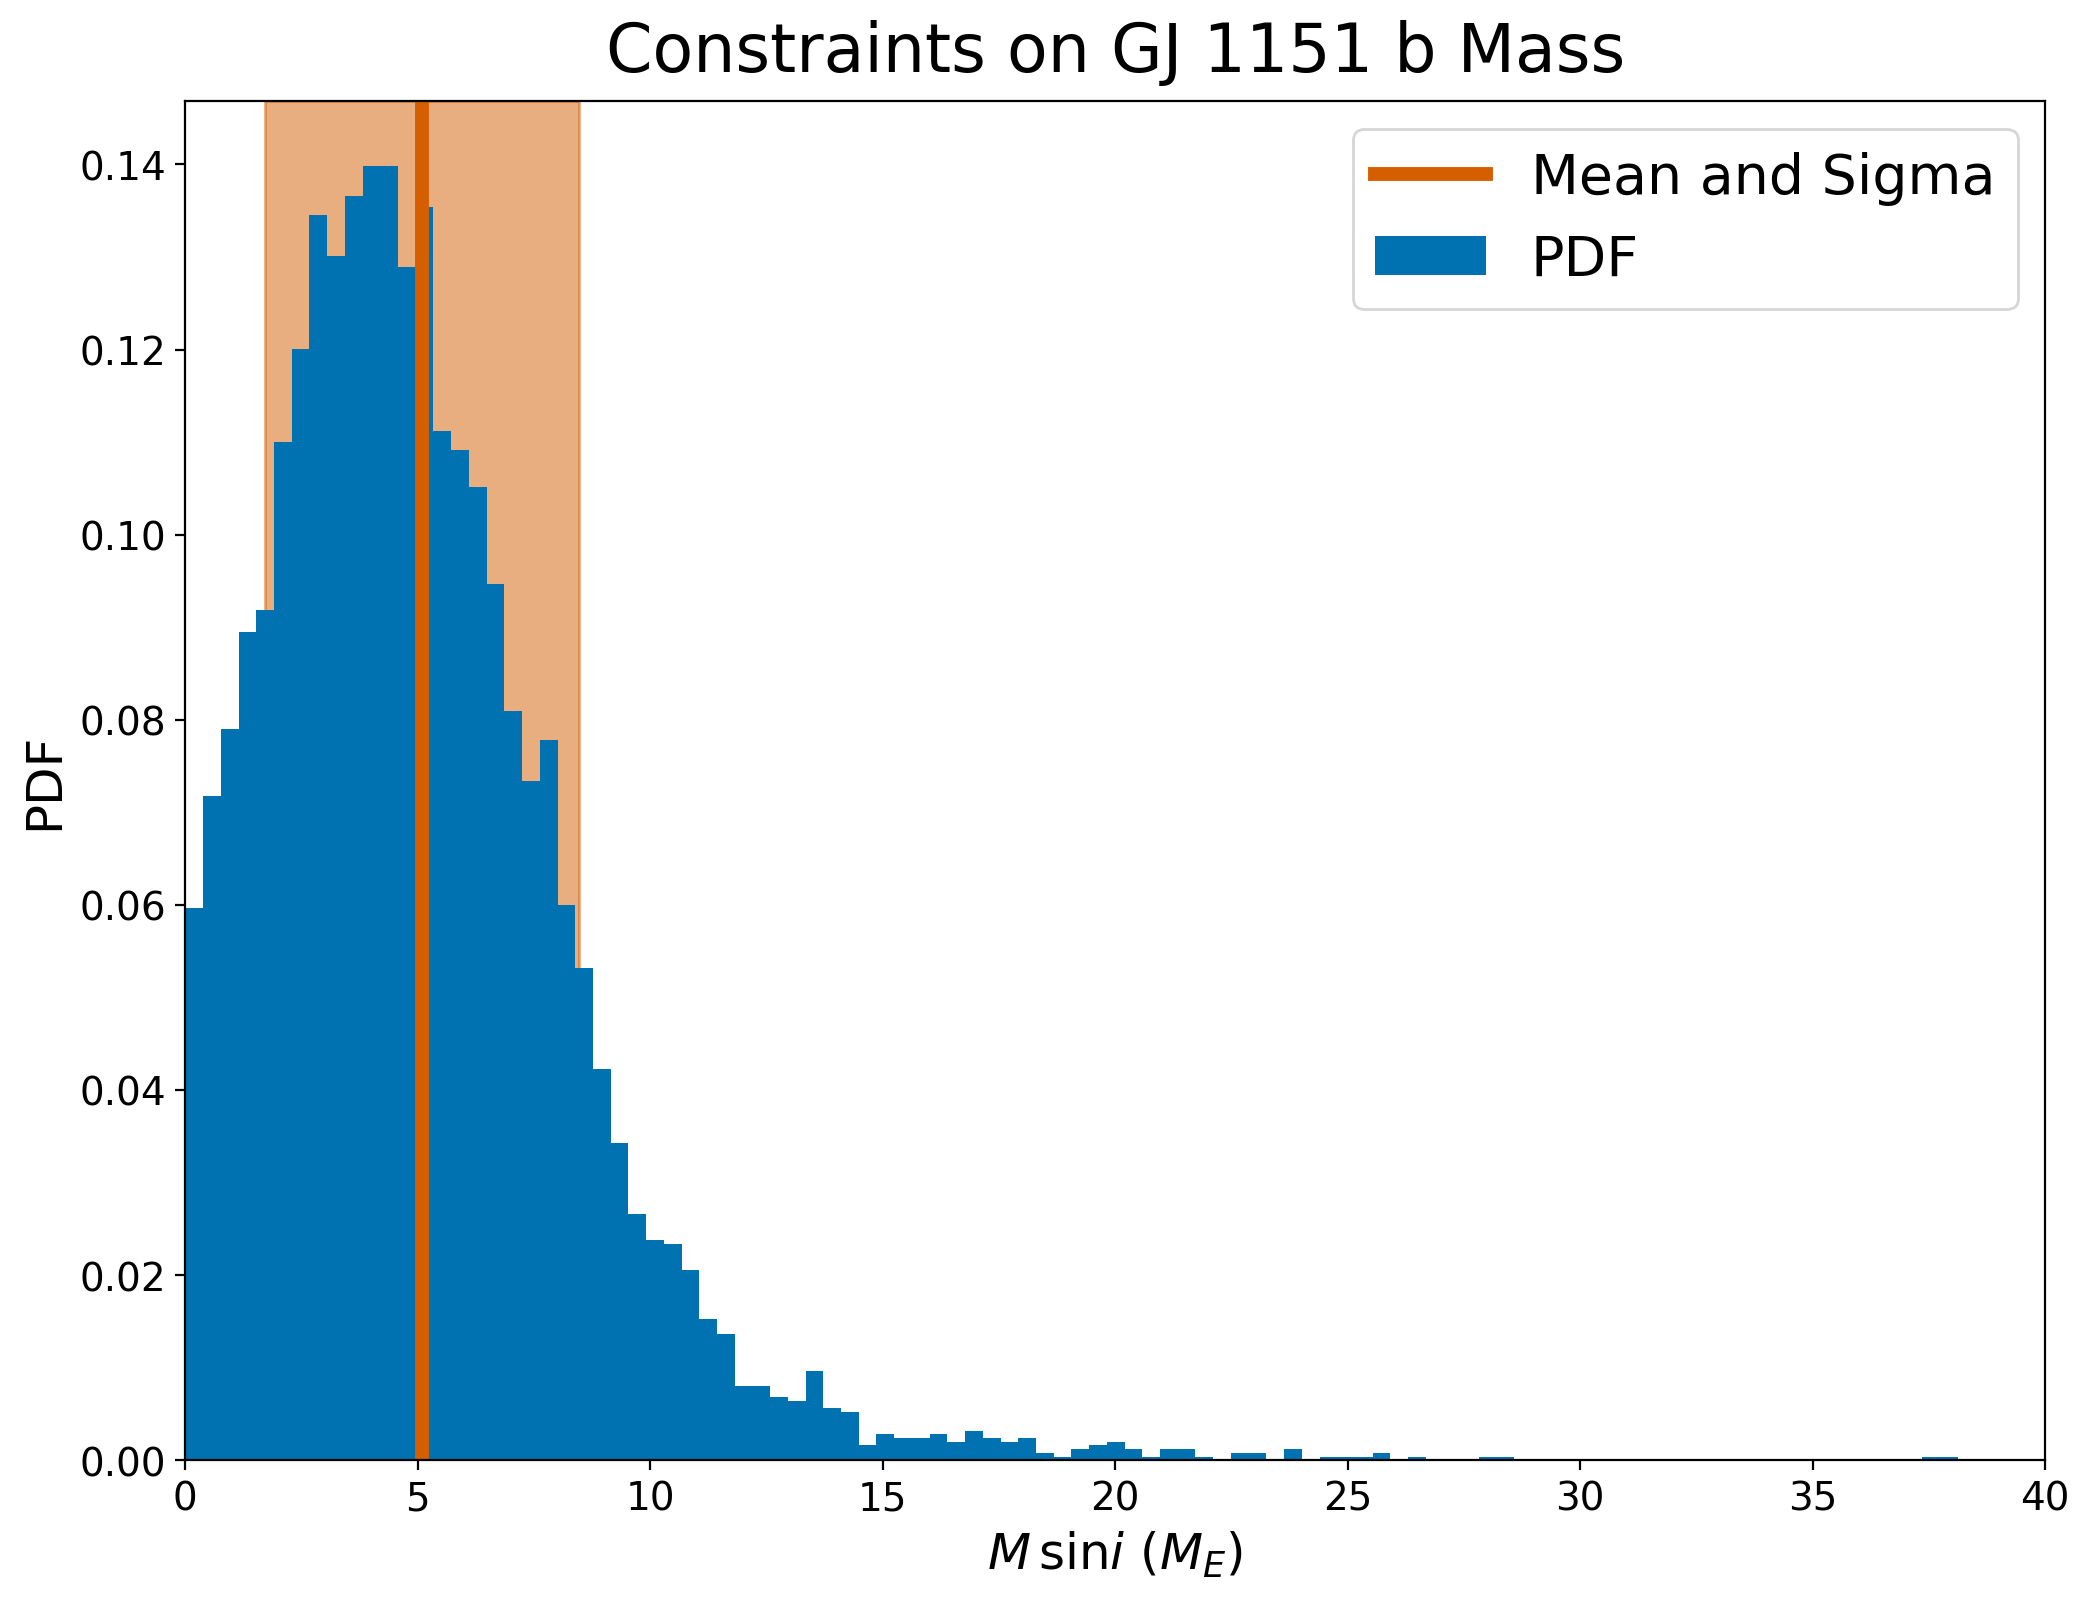
\includegraphics[width=15cm,keepaspectratio]{gj1151b_mass.png}

\caption{\label{mass}
Planet mass posterior.
}
\end{figure}

\section{Discussion}
\label{sec:discussion}

\section{Conclusions}
\label{sec:conclusions}

\section*{Acknowledgements} % add your acknowledgements text here!

This work was performed in part under contract with the Jet Propulsion Laboratory (JPL) funded by NASA through the Sagan Fellowship Program executed by the NASA Exoplanet Science Institute. TRW acknowledges the support of the Australian Research Council (grant DP150100250) and the Villum Foundation (research grant 10118). 

BJSP acknowledges being on the traditional territory of the Lenape Nations and recognizes that Manhattan continues to be the home to many Algonkian peoples. We give blessings and thanks to the Lenape people and Lenape Nations in recognition that we are carrying out this work on their indigenous homelands.
%

This research made use of NASA's Astrophysics Data System; the SIMBAD database, operated at CDS, Strasbourg, France; the IPython package \citep{PER-GRA:2007}; SciPy \citep{scipy}; and Astropy, a community-developed core Python package for Astronomy \citep{astropy}. Some of the data presented in this paper were obtained from the Mikulski Archive for Space Telescopes (MAST). STScI is operated by the Association of Universities for Research in Astronomy, Inc., under NASA contract NAS5-26555. Support for MAST for non-HST data is provided by the NASA Office of Space Science via grant NNX13AC07G and by other grants and contracts. 

%%%%%%%%%%%%%%%%%%%%%%%%%%%%%%%%%%%%%%%%%%%%%%%%%%

%%%%%%%%%%%%%%%%%%%% REFERENCES %%%%%%%%%%%%%%%%%%


\bibliography{ms}


%% This command is needed to show the entire author+affilation list when
%% the collaboration and author truncation commands are used.  It has to
%% go at the end of the manuscript.
%\allauthors

%% Include this line if you are using the \added, \replaced, \deleted
%% commands to see a summary list of all changes at the end of the article.
%\listofchanges

\end{document}

% End of file `sample62.tex'.
